\documentclass[8pt]{beamer}

% Beamer style
%\usetheme[secheader]{Madrid}
% \usetheme{CambridgeUS}
\useoutertheme{infolines}
\usecolortheme[rgb={0.65,0.15,0.25}]{structure}
% \usefonttheme[onlymath]{serif}
\beamertemplatenavigationsymbolsempty
%\AtBeginSubsection

% Packagesg
%\usepackage[french]{babel}
\usepackage[latin1]{inputenc}
\usepackage{color}
\usepackage{xspace}
\usepackage{enumerate}
\usepackage{dsfont, stmaryrd}
% \usepackage{amsmath, amsfonts, amssymb}
\usepackage{amsmath, amsfonts, amssymb, MnSymbol}
\usepackage{epsfig}
\usepackage{tikz}
\usepackage{url}
\usepackage{/home/robin/LATEX/Biblio/astats}
%\usepackage[all]{xy}
\usepackage{graphicx}

% Commands
% Maths
% \newtheorem{theorem}{Theorem}
% \newtheorem{definition}{Definition}
\newtheorem{proposition}{Proposition}
% \newtheorem{assumption}{Assumption}
% \newtheorem{algorithm}{Algorithm}
% \newtheorem{lemma}{Lemma}
% \newtheorem{remark}{Remark}
% \newtheorem{exercise}{Exercise}
% \newcommand{\propname}{Prop.}
% \newcommand{\proof}{\noindent{\sl Proof:}\quad}
% \newcommand{\eproof}{$\blacksquare$}

% \setcounter{secnumdepth}{3}
% \setcounter{tocdepth}{3}
\newcommand{\pref}[1]{\ref{#1} p.\pageref{#1}}
\newcommand{\qref}[1]{\eqref{#1} p.\pageref{#1}}

% Colors : http://latexcolor.com/
\definecolor{darkred}{rgb}{0.65,0.15,0.25}
\definecolor{darkgreen}{rgb}{0,0.4,0}
\definecolor{darkred}{rgb}{0.65,0.15,0.25}
\definecolor{amethyst}{rgb}{0.6, 0.4, 0.8}
\definecolor{asparagus}{rgb}{0.53, 0.66, 0.42}
\definecolor{applegreen}{rgb}{0.55, 0.71, 0.0}
\definecolor{awesome}{rgb}{1.0, 0.13, 0.32}
\definecolor{blue-green}{rgb}{0.0, 0.87, 0.87}
\definecolor{red-ggplot}{rgb}{0.52, 0.25, 0.23}
\definecolor{green-ggplot}{rgb}{0.42, 0.58, 0.00}
\definecolor{purple-ggplot}{rgb}{0.34, 0.21, 0.44}
\definecolor{blue-ggplot}{rgb}{0.00, 0.49, 0.51}

% Commands
\newcommand{\backupbegin}{
   \newcounter{finalframe}
   \setcounter{finalframe}{\value{framenumber}}
}
\newcommand{\backupend}{
   \setcounter{framenumber}{\value{finalframe}}
}
\newcommand{\emphase}[1]{\textcolor{darkred}{#1}}
\newcommand{\comment}[1]{\textcolor{gray}{#1}}
\newcommand{\paragraph}[1]{\textcolor{darkred}{#1}}
\newcommand{\refer}[1]{{\small{\textcolor{gray}{{\cite{#1}}}}}}
\newcommand{\Refer}[1]{{\small{\textcolor{gray}{{[#1]}}}}}
\newcommand{\goto}[1]{{\small{\textcolor{blue}{[\#\ref{#1}]}}}}
\renewcommand{\newblock}{}

\newcommand{\tabequation}[1]{{\medskip \centerline{#1} \medskip}}
% \renewcommand{\binom}[2]{{\left(\begin{array}{c} #1 \\ #2 \end{array}\right)}}

% Variables 
\newcommand{\Abf}{{\bf A}}
\newcommand{\Beta}{\text{B}}
\newcommand{\Bcal}{\mathcal{B}}
\newcommand{\Bias}{\xspace\mathbb B}
\newcommand{\Cor}{{\mathbb C}\text{or}}
\newcommand{\Cov}{{\mathbb C}\text{ov}}
\newcommand{\cl}{\text{\it c}\ell}
\newcommand{\Ccal}{\mathcal{C}}
\newcommand{\cst}{\text{cst}}
\newcommand{\Dcal}{\mathcal{D}}
\newcommand{\Ecal}{\mathcal{E}}
\newcommand{\Esp}{\xspace\mathbb E}
\newcommand{\Espt}{\widetilde{\Esp}}
\newcommand{\Covt}{\widetilde{\Cov}}
\newcommand{\Ibb}{\mathbb I}
\newcommand{\Fcal}{\mathcal{F}}
\newcommand{\Gcal}{\mathcal{G}}
\newcommand{\Gam}{\mathcal{G}\text{am}}
\newcommand{\Hcal}{\mathcal{H}}
\newcommand{\Jcal}{\mathcal{J}}
\newcommand{\Lcal}{\mathcal{L}}
\newcommand{\Mt}{\widetilde{M}}
\newcommand{\mt}{\widetilde{m}}
\newcommand{\Nbb}{\mathbb{N}}
\newcommand{\Mcal}{\mathcal{M}}
\newcommand{\Ncal}{\mathcal{N}}
\newcommand{\Ocal}{\mathcal{O}}
\newcommand{\pt}{\widetilde{p}}
\newcommand{\Pt}{\widetilde{P}}
\newcommand{\Pbb}{\mathbb{P}}
\newcommand{\Pcal}{\mathcal{P}}
\newcommand{\Qcal}{\mathcal{Q}}
\newcommand{\qt}{\widetilde{q}}
\newcommand{\Rbb}{\mathbb{R}}
\newcommand{\Sbb}{\mathbb{S}}
\newcommand{\Scal}{\mathcal{S}}
\newcommand{\st}{\widetilde{s}}
\newcommand{\St}{\widetilde{S}}
\newcommand{\Tcal}{\mathcal{T}}
\newcommand{\todo}{\textcolor{red}{TO DO}}
\newcommand{\Ucal}{\mathcal{U}}
\newcommand{\Un}{\math{1}}
\newcommand{\Vcal}{\mathcal{V}}
\newcommand{\Var}{\mathbb V}
\newcommand{\Vart}{\widetilde{\Var}}
\newcommand{\Zcal}{\mathcal{Z}}

% Symboles & notations
\newcommand\independent{\protect\mathpalette{\protect\independenT}{\perp}}\def\independenT#1#2{\mathrel{\rlap{$#1#2$}\mkern2mu{#1#2}}} 
\renewcommand{\d}{\text{\xspace d}}
\newcommand{\gv}{\mid}
\newcommand{\ggv}{\, \| \, }
% \newcommand{\diag}{\text{diag}}
\newcommand{\card}[1]{\text{card}\left(#1\right)}
\newcommand{\trace}[1]{\text{tr}\left(#1\right)}
\newcommand{\matr}[1]{\boldsymbol{#1}}
\newcommand{\matrbf}[1]{\mathbf{#1}}
\newcommand{\vect}[1]{\matr{#1}} %% un peu inutile
\newcommand{\vectbf}[1]{\matrbf{#1}} %% un peu inutile
\newcommand{\trans}{\intercal}
\newcommand{\transpose}[1]{\matr{#1}^\trans}
\newcommand{\crossprod}[2]{\transpose{#1} \matr{#2}}
\newcommand{\tcrossprod}[2]{\matr{#1} \transpose{#2}}
\newcommand{\matprod}[2]{\matr{#1} \matr{#2}}
\DeclareMathOperator*{\argmin}{arg\,min}
\DeclareMathOperator*{\argmax}{arg\,max}
\DeclareMathOperator{\sign}{sign}
\DeclareMathOperator{\tr}{tr}
\newcommand{\ra}{\emphase{$\rightarrow$} \xspace}

% Hadamard, Kronecker and vec operators
\DeclareMathOperator{\Diag}{Diag} % matrix diagonal
\DeclareMathOperator{\diag}{diag} % vector diagonal
\DeclareMathOperator{\mtov}{vec} % matrix to vector
\newcommand{\kro}{\otimes} % Kronecker product
\newcommand{\had}{\odot}   % Hadamard product

% TikZ
\newcommand{\nodesize}{2em}
\newcommand{\edgeunit}{2.5*\nodesize}
\newcommand{\edgewidth}{1pt}
\tikzstyle{node}=[draw, circle, fill=black, minimum width=.75\nodesize, inner sep=0]
\tikzstyle{square}=[rectangle, draw]
\tikzstyle{param}=[draw, rectangle, fill=gray!50, minimum width=\nodesize, minimum height=\nodesize, inner sep=0]
\tikzstyle{hidden}=[draw, circle, fill=gray!50, minimum width=\nodesize, inner sep=0]
\tikzstyle{hiddenred}=[draw, circle, color=red, fill=gray!50, minimum width=\nodesize, inner sep=0]
\tikzstyle{observed}=[draw, circle, minimum width=\nodesize, inner sep=0]
\tikzstyle{observedred}=[draw, circle, minimum width=\nodesize, color=red, inner sep=0]
\tikzstyle{eliminated}=[draw, circle, minimum width=\nodesize, color=gray!50, inner sep=0]
\tikzstyle{empty}=[draw, circle, minimum width=\nodesize, color=white, inner sep=0]
\tikzstyle{blank}=[color=white]
\tikzstyle{nocircle}=[minimum width=\nodesize, inner sep=0]

\tikzstyle{edge}=[-, line width=\edgewidth]
\tikzstyle{edgebendleft}=[-, >=latex, line width=\edgewidth, bend left]
\tikzstyle{edgebendright}=[-, >=latex, line width=\edgewidth, bend right]
\tikzstyle{lightedge}=[-, line width=\edgewidth, color=gray!50]
\tikzstyle{lightedgebendleft}=[-, >=latex, line width=\edgewidth, bend left, color=gray!50]
\tikzstyle{lightedgebendright}=[-, >=latex, line width=\edgewidth, bend right, color=gray!50]
\tikzstyle{edgered}=[-, line width=\edgewidth, color=red]
\tikzstyle{edgebendleftred}=[-, >=latex, line width=\edgewidth, bend left, color=red]
\tikzstyle{edgebendrightred}=[-, >=latex, line width=\edgewidth, bend right, color=red]

\tikzstyle{arrow}=[->, >=latex, line width=\edgewidth]
\tikzstyle{arrowbendleft}=[->, >=latex, line width=\edgewidth, bend left]
\tikzstyle{arrowbendright}=[->, >=latex, line width=\edgewidth, bend right]
\tikzstyle{arrowred}=[->, >=latex, line width=\edgewidth, color=red]
\tikzstyle{arrowbendleftred}=[->, >=latex, line width=\edgewidth, bend left, color=red]
\tikzstyle{arrowbendrightred}=[->, >=latex, line width=\edgewidth, bend right, color=red]
\tikzstyle{arrowblue}=[->, >=latex, line width=\edgewidth, color=blue]
\tikzstyle{dashedarrow}=[->, >=latex, dashed, line width=\edgewidth]
\tikzstyle{dashededge}=[-, >=latex, dashed, line width=\edgewidth]
\tikzstyle{dashededgebendleft}=[-, >=latex, dashed, line width=\edgewidth, bend left]
\tikzstyle{lightarrow}=[->, >=latex, line width=\edgewidth, color=gray!50]


% Directory
% \newcommand{\figpaper}{/home/robin/Bureau/Dropbox/VBEM-IS/Article_New/plots}
\newcommand{\fignet}{/home/robin/RECHERCHE/RESEAUX/EXPOSES/FIGURES}
\newcommand{\figtree}{/home/robin/RECHERCHE/BAYES/VBEM-IS/VBEM-IS.git/Data/Tree/Fig}
\newcommand{\figbayes}{/home/robin/RECHERCHE/BAYES/EXPOSES/FIGURES}
\newcommand{\figzebra}{/home/robin/RECHERCHE/BAYES/VBEM-IS/VBEM-IS.git/Data/Zebra/Fig}

%====================================================================
%====================================================================

%====================================================================
%====================================================================
\begin{document}
%====================================================================
%====================================================================

%====================================================================
\title[SMC sampling for Poisson SBM]{SMC sampling from deterministic approximations: \\ ~\\ Application to the Poisson stochastic block-model}

\author[S. Robin]{S. Robin \\ ~\\
    Joint work with \underline{S. Donnet}
  }

\institute[]{Sorbonne universit\'e \\ ~ \\
Laboratoire de Probabilit\'es, Statistique et Mod\'elisation (LPSM)}

\date[Dec.'22, London]{CMStatistics, December 2022, London}

%====================================================================
%====================================================================
\maketitle
%====================================================================

%====================================================================
%====================================================================
\section{Motivating example}
\frame{\frametitle{Outline} \tableofcontents[currentsection]}
%====================================================================
\frame{\frametitle{Motivating example}

%   \paragraph{Data at hand.} ~ \\
  \begin{tabular}{ccc}
  Interaction network & \multicolumn{2}{c}{Edge covariates} \\
  \includegraphics[width=.3\textwidth]{\figbayes/FigVBEM-IS-Tree-Network}   
  &
  \includegraphics[width=.3\textwidth]{\figbayes/FigVBEM-IS-Tree-TaxonomicDistance.pdf}
  &
  \includegraphics[width=.3\textwidth]{\figbayes/FigVBEM-IS-Tree-GeographicDistance.pdf} 
  \\
  \multicolumn{3}{l}{$Y_{ij} =$ number of interactions between nodes $i$ and $j$ (count)}
  \end{tabular}

  \bigskip \bigskip \pause
  \paragraph{Questions.}
  \begin{itemize}
   \item Is there some structure in the network?
   \item Do the covariates contribute to explain it?
   \item Do they explain all of the structure? Is there some 'residual' structure?
  \end{itemize}
}

%====================================================================
\frame{\frametitle{Stochastic block-model (SBM)}

  \paragraph{Proposed model.} 
  Poisson SBM, including covariates \refer{MRV10}
  
  \bigskip \pause
  \begin{tabular}{cc}
    \onslide+<1->{
    \begin{tabular}{p{.5\textwidth}}
    \paragraph{Frequentist version.} \\
    ~ \\
    $n$ nodes ($1 \leq i, j \leq n$) \\
    ~ \\
    $\{Z_i\}_i$ iid $\sim \Mcal_K(1, \pi)$ \\
    ~ \\
    $\{Y_{ij}\}_{i < j}$ independent $\mid \{Z_i\}$ \\
    ~ \\
    $Y_{ij} \mid \emphase{(Z_i = k, Z_j = \ell)}
    \sim \Pcal(\exp(\alpha_{k\ell} + x_{ij}^\trans \beta))$
    \end{tabular}
    }
    & 
    \onslide+<3>{
    \begin{tabular}{p{.5\textwidth}}
    \paragraph{Bayesian version.} \\
    ~ \\ ~ \\ ~ \\
    $\pi \sim \Dcal_K(a)$ \\
    ~ \\ ~ \\ ~ \\
    $\gamma = (\alpha, \beta) \sim \Ncal(\gamma_0, V_0)$
    \end{tabular}
    }
  \end{tabular}

  \onslide+<2->{
  \bigskip \bigskip
  \paragraph{Latent variables $Z$, parameter $\theta = (\pi, \alpha, \beta)$.}
  \begin{align*}
    Z = \{Z_i\} & = \text{ node memberships}
    & 
    \pi & = \text{ group proportions} \\
    \alpha & = \text{ between group interactions}
    & 
   \beta & = \text{ effects of the covariates}
  \end{align*}
  }

}

%====================================================================
\frame{\frametitle{Inference of SBM}

  \begin{itemize}
   \item Bayesian inference using MCMC: time consuming + convergence issues \\
   ~ \\
   \item Frequenstist inference via maximum likelihood (ML): intractable \\
   ~ \\
   \item Variational approximation of ML (VEM): efficient, but with no statistical guaranty \\
   ~ \\
   \item No easy-to-handle variational Bayes approximation (no conjugacy)
  \end{itemize}

  \bigskip \bigskip \pause
  \paragraph{Aim.}
  \begin{itemize}
   \item Design an efficient posterior sampling algorithm taking advantage of the efficiency of (frequentist) VEM inference
  \end{itemize}

}

%====================================================================
%====================================================================
\section{Variational EM inference}
\frame{\frametitle{Outline} \tableofcontents[currentsection]}
%====================================================================
\frame{\frametitle{EM and VEM}

  SBM = incomplete data model
  
  \bigskip \bigskip
  \paragraph{Maximum likelihood.} Most popular way: EM
  $$
  \log p_\theta(Y) 
  = \Esp\left((\log p_\theta(Y, Z) \mid Y\right) - \Esp\left(\log p_\theta(Z \mid Y) \mid Y \right)
  $$
  \ra Requires to determine (some moments of) $p_\theta(Z \mid Y)$, which is intractable.
  
  \bigskip \bigskip \pause
  \paragraph{Variational approximation.} When $p_\theta(Z \mid Y)$ is intractable, rather maximize the ELBO
  \begin{align*}
   J(\theta, q) 
   & = \log p_\theta(Y) - KL\left(q(Z) \| p_\theta(Z \mid Y) \right) \\
   & = \Esp_{\emphase{q}}\log p_\theta(Y, Z) - \Esp_{\emphase{q}}\log q(Z) \leq \log p_\theta(Y)
  \end{align*}
  taking $q \in \Qcal$. 
  
  \bigskip \bigskip 
  \paragraph{Mean field.} Typical choice for SBM: $\Qcal = \left\{ q: q(Z) = \prod_i q_i(Z_i) \right\}$ 
  ({\tt Blockmodels} \refer{Leg16}).
  
}

%====================================================================
\frame{\frametitle{Approximate posterior}

  \paragraph{Taylor expansion.} Denote $(\widetilde{\theta}, \qt) = \arg\max_{\theta, q \in \Qcal} J(\theta, q)$ and approximate 
  \begin{align*}
    \log p(\theta \mid Y)
    & \propto \exp \left(\log \pi(\theta) + \log p_\theta(Y) \right) 
    \emphase{\simeq} \exp \left(\log \pi(\theta) + J(\theta, \qt) \right) \\
    & \emphase{\simeq} \exp \left(\log \pi(\theta) + J(\widetilde{\theta}, \qt) + \frac12 (\theta - \widetilde{\theta})^\top \partial_{\theta^2}J(\theta, \qt) (\theta - \widetilde{\theta}) \right)
  \end{align*}
    
  \bigskip \pause
  \paragraph{Variance proxy for VEM estimates.} 
  Set $\widetilde{V}_\gamma := - \left(\partial_{\gamma^2}J(\theta, \qt)\right)^{-1}$ and use conjugacy rules to get
  \begin{align*}
    \widetilde{\Var}(\gamma) 
    & = \left(V_0^{-1} + \widetilde{V}_\gamma^{-1}\right)^{-1}, &
    \widetilde{\Esp}(\gamma) 
    & = \widetilde{\Var}(\gamma)^{-1} \left(V_0^{-1} \gamma_0 + \widetilde{V}_\gamma^{-1} \widetilde{\gamma}\right)^{-1}
  \end{align*}
  and define
  $$
  \pt(\gamma) := \Ncal\left(\widetilde{\Esp}(\gamma), \widetilde{\Var}(\gamma)\right) \qquad \simeq p(\gamma \mid Y).
  $$
  
  \bigskip \bigskip \pause
  \paragraph{Approximate posterior.} 
  Proceed similarly to define $\widetilde{a}$ and set
  $$
  \pt(\gamma) := \Dcal(\widetilde{a}) \qquad \simeq p(\pi \mid Y),
  $$
  then combine the two
  $$
  \pt(\theta) := \pt(\pi) \pt(\gamma) \qquad \simeq p(\theta \mid Y).
  $$
}

%====================================================================
\section{SMC sampling}
\frame{\frametitle{Outline} \tableofcontents[currentsection]}
%====================================================================
\frame{\frametitle{Sampling principle}  

  \begin{tabular}{cc}
    \begin{tabular}{p{.5\textwidth}}
	 \begin{itemize}
	   \onslide+<1->{\item $\textcolor{red}{p_0} = $ proposal, $\textcolor{blue}{p^*} = $ target \\ ~ \\}	 
	   \onslide+<2->{\item Intermediate distributions
		$$
		p_0, p_1, ..., p_H = p^*
		$$
		~ \\
		}	 
	   \onslide+<3->{\item Iteratively: \\
	   use $p_h$ to get a sample from $p_{h+1}$}
	 \end{itemize}
    \end{tabular}
    & 
    \hspace{-.02\textwidth}
    \begin{tabular}{p{.5\textwidth}}
 	 \begin{overprint}
 	   \onslide<1> 
 	   \includegraphics[width=.4\textwidth]{\figbayes/FigVBEM-IS-PropTarget.pdf}
 	   \onslide<2> 
 	   \includegraphics[width=.4\textwidth]{\figbayes/FigVBEM-IS-Tempering.pdf}
 	   \onslide<3> 
 	   \includegraphics[width=.4\textwidth]{\figbayes/FigVBEM-IS-Tempering-step1.pdf}
 	   \onslide<4> 
 	   \includegraphics[width=.4\textwidth]{\figbayes/FigVBEM-IS-Tempering-step2.pdf}
 	   \onslide<5> 
 	   \includegraphics[width=.4\textwidth]{\figbayes/FigVBEM-IS-Tempering-step3.pdf}
 	   \onslide<6-> 
 	   \includegraphics[width=.4\textwidth]{\figbayes/FigVBEM-IS-Tempering-step4.pdf}
 	 \end{overprint}
    \end{tabular}
  \end{tabular}
  

  \onslide+<7>{
    \bigskip 
    \paragraph{Here.}
    Take $p_0 = \pt$ (rather than $p_0 = \pi =$ prior), $p^* = p(\cdot \mid Y)$ 
    }

}
  
%====================================================================
\frame{\frametitle{Sequential importance sampling scheme}

  Denote
  $$
  \emphase{U = (\theta, Z)}, \qquad
  \pi = \text{ prior}, \qquad
  \ell = \text{ likelihood}
  $$

  \bigskip
  \paragraph{Distribution path:} 
    set $0 = \rho_0 < \rho_1 < \dots < \rho_{H-1} < \rho_H = 1$,
  \begin{align*}
     p_h(U) & \propto \pt(U)^{\emphase{{1-\rho_h}}} \; \times \; p(U | Y)^{\emphase{{\rho_h}}} \\
%      \\
     & \propto \pt(U) \; \times \; r(U)^{\emphase{{\rho_h}}}, 
     & r(U) & = \frac{\pi(U) \ell(Y | U)}{\pt(U)}
  \end{align*}
  
  \bigskip \bigskip \pause
  \paragraph{Sequential sampling.} At each step $h$, provides
  $$
  \Ecal_h = \{(U_h^m, w_h^m)\}_m = \text{ weighted sample of } p_h
  $$

  \bigskip \pause
  \paragraph{Question.} 
  How to tune $\{\rho_h\}$ or $H$ to keep each sampling step efficient?

}
  
%====================================================================
\frame{\frametitle{Proposed algorithm}

  \begin{description}
   \item[Init.:] Sample $(U_0^m)_m$ iid $\sim \pt$, $w_0^m = 1$ \\ ~
   \pause
   \item[Step $h$:] Using the previous sample $\Ecal_{h-1} = \{(U_{h-1}^m, w_{h-1}^m)\}$ \\ ~
   \pause
   \begin{enumerate}
    \item compute $w_h^m = w_{h-1}^m \times (r_{\emphase{h-1}}^m)^{\rho_h - \rho_{h-1}}$ \\
    tuning $\rho_h$ so that $cESS(\Ecal_{h-1}; p_{h-1}, p_h) = \emphase{\tau_1}$ \\ ~
    \pause
    \item (\footnote{To avoid degeneracy. Weights set to 1 after it.}) if $ESS_h = \overline{w}_h^2 / \overline{w_h^2} < \emphase{\tau_2}$, resample the particles  \\ ~
    \pause
    \item (\footnote{$K_h$ has stationary distribution \emphase{$p_h$} (e.g. Gibbs sampler). Only propagation: no convergence needed}) propagate the particles $U_h^m \sim \emphase{K_h}(U_h^m | U_{h-1}^m)$ 
   \end{enumerate} ~ 
   \pause
   \item[Stop:] When $\rho_h$ reaches 1.
  \end{description}
  

}
  
%====================================================================
\frame{\frametitle{Some comments}

  \paragraph{Justification of the algorithm \refer{DDJ06}.} At each step $h$, construct a distribution for the whole particle path with marginal $p_h$.

  \bigskip \bigskip \bigskip \pause
  \paragraph{Conditional ESS.} Efficiency of sample $\Ecal$ from $p_{h-1}$ for distribution $p_h$
%   $$
%   cESS(\Ecal; q, p) = \frac{M \left(\sum_m W^m a^m\right)^2}{\sum_m W^m (a^m)^2}, 
%   \qquad a^m = \frac{p(U^m)}{q(U^m)}
%   $$
%   \ra Step 1: find next $p_h$ s.t. sample $\Ecal_{h-1}$ is reasonably efficient.
%   
% %   \bigskip \bigskip \bigskip \pause
% %   \paragraph{ESS:} intrinsic efficiency of a sample 
% %   $$
% %   ESS(\{(U^m, w^m)\}) = \frac{M \left(\sum_m w^m\right)^2}{\sum_m (w^m)^2}
% %   $$
% %   \ra Step 1c: resample if to few particles actually contribute
%   
%   \bigskip \bigskip \pause
%   Update formula of the weights
  $$
  cESS(\Ecal_{h-1}; p_{h-1}, p_h) 
  = 
  \frac
  {M \left[\sum_m W_{h-1}^m \; (\emphase{r^m_{h-1}})^{\rho_h -\rho_{h-1}}\right]^2}
  {\sum_m W_{h-1}^m \; (\emphase{r^m_{h-1}})^{2\rho_h - 2\rho_{h-1}}}
  $$
  \begin{itemize}
    \item Can be computed for any $\rho_h$ \emphase{before sampling}.
    \item $\rho_h$ tuned to meet $\tau_1$, which controls the step size $\rho_h - \rho_{h-1}$ (and $H$)

  \end{itemize}
  
  \bigskip \bigskip \bigskip \pause
  \paragraph{Marginal likelihood.} An estimate of the marginal likelihoog $p(Y)$ is also available as a side product.
}

%====================================================================
\frame{\frametitle{Variational approximation vs prior}

  Starting from $p_0 = \pt$ reduces the number of SMC steps wrt starting from $p_0 = \pi$.
  $$
  \includegraphics[width=.5\textwidth]{\figbayes/DoR21-Fig1-simu-rho} 
  $$
  (synthetic data)
}
  
%====================================================================
\section{Illustrations}
\subsection*{Tree network}
\frame{\frametitle{Outline} \tableofcontents[currentsection]}

%====================================================================
\frame{\frametitle{Tree network}

  \begin{tabular}{ll}
   \begin{tabular}{p{.4\textwidth}}
    \paragraph{From \refer{VPD08}.} \\
    ~ \\ ~ \\
    $n = 51$ tree species \\
    ~ \\ ~ \\
    3 covariates (distances): \\
    taxonomy, geography, genetics \\
    ~ \\ ~ \\ 
    $Y_{ij} = $ number of shared fungal parasites \\
    ~ \\

   \end{tabular}
   &
   \hspace{-.1\textwidth}
   \begin{tabular}{p{.5\textwidth}}
    \includegraphics[width=.5\textwidth]{\figbayes/FigVBEM-IS-Tree-Network} 
   \end{tabular}
  \end{tabular}

}

%====================================================================
\frame{\frametitle{Sampling path \& choice of $K$}

  \paragraph{Full model.} All covariates

  \bigskip
  \begin{center}
    \begin{tabular}{ccc}
    Model selection & & Sampling path: $\rho_h$ \\
    \includegraphics[width=.3\textwidth]{\figbayes/DoR21-Fig7-logpY} &
    \qquad &
    \includegraphics[width=.3\textwidth]{\figbayes/DoR21-Fig7-rho} \\
    \textcolor{orange}{$J_K$}, \textcolor{darkgreen}{$\log (Y \mid K)$}, \textcolor{purple}{$\widetilde{ICL}(K)$} 
    \end{tabular}
  \end{center}
  
  \bigskip \bigskip
  \paragraph{Choosing the number of groups:} $\widehat{K} = \arg\max_K \widehat{p}(K \mid Y)$ 
  \begin{itemize}
    \item Different from $\arg\max_K \widetilde{ICL}(K)$ here.
  \end{itemize}
}

%====================================================================
\frame{\frametitle{Posterior distribution of $\beta$}

  \vspace{-.05\textheight}
  \begin{center}
    \begin{tabular}{ccc}
    taxonomy & geography & genetics \\
    \includegraphics[width=.3\textwidth]{\figbayes/DoR21-Fig7-beta1} & 
    \includegraphics[width=.3\textwidth]{\figbayes/DoR21-Fig7-beta2} & 
    \includegraphics[width=.3\textwidth]{\figbayes/DoR21-Fig7-beta3} \\
    \multicolumn{3}{c}{\textcolor{orange}{$\pt(\beta \mid \widehat{K})$}, \quad  \textcolor{darkgreen}{$\widehat{p}(\beta \mid Y, \widehat{K})$}, \quad \textcolor{purple}{$\widehat{p}(\beta \mid Y) = \sum_K \widehat{p}(K \mid Y) \widehat{p}(\beta \mid Y, K)$}}
    \end{tabular}
  \end{center}  

  \bigskip \pause
  \hspace{-.025\textwidth}
  \begin{tabular}{rrrr}
    \paragraph{Correlation between estimates.} 
    & $(\beta_1, \beta_2)$ & $(\beta_1, \beta_3)$ & $(\beta_2, \beta_3)$ \\
    $\pt(\beta)$    & $-0.012$ & $ 0.021$ & $ 0.318$ \\
    $\widehat{p}(\beta \mid Y)$ & $-0.274$ & $-0.079$ & $-0.088$
  \end{tabular}

  \bigskip \bigskip 
  \paragraph{Model selection.} 
  $
  \widehat{P}\{x = \text{(taxo., geo.)} \mid Y \} \simeq 70\%, \quad
  \widehat{P}\{x = \text{(taxo.)} \mid Y \} \simeq 30\%
  $
}

%====================================================================
\frame{\frametitle{Residual structure}

  Between group interactions ($\alpha_{k\ell}$) = 'residuals' = not explained by the covariates.

  \pause
  \hspace{-.05\textwidth}
  \begin{tabular}{cc}
    \begin{tabular}{p{.4\textwidth}}
      \paragraph{'Graphon' representation.} \refer{LRO17} \\
      Group interactions encoded as
      $$
      \phi: [0, 1]^2 \mapsto \Rbb
      $$
      \begin{itemize}
       \item symmetric\footnote{with increasing marginal $\overline{\phi}(u) = \int \phi(u, v) \d v$ to ensure identifiability.}, 
       \item block-wise constant, 
       \item block width $= \pi_k$
       \item block height $= \alpha_{k\ell}$
      \end{itemize}
    \end{tabular}
    & 
    \begin{tabular}{p{.5\textwidth}}
      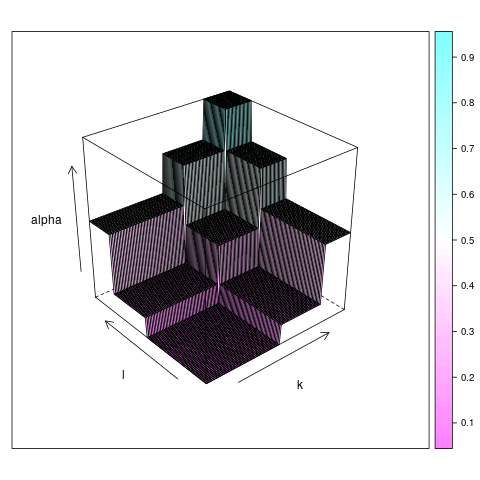
\includegraphics[trim=50 50 50 50, width=.5\textwidth, clip=T]{\fignet/FigGraphon-SBM-graphon-alpha}
    \end{tabular}
  \end{tabular}
  
%   \vspace{-.1\textheight}
  \pause 
  \paragraph{Same representation for all $K$.}
  $
  Y_{ij} | (U_i, U_j) \sim \Pcal\left(\exp(\phi(U_i, U_j) + x_{ij}^\trans \beta \right)
  $
  
  }

%====================================================================
\frame{\frametitle{Tree network residual structure}

%   \vspace{-.2\textheight}
  \hspace{-.04\textwidth}
  \begin{tabular}{cc}
    \begin{tabular}{p{.4\textwidth}}
      \paragraph{Residual graphon.} \\
      Each particle $\theta^m$ provides an estimate of $\phi^m(u, v)$ \\
      ~ \\
      ~ \\
      All estimates can be averaged (over both $m$ and $K$)
    \end{tabular}
    & 
    \pause
%     \hspace{-.05\textwidth}
    \begin{tabular}{p{.5\textwidth}}
    \includegraphics[trim=130 120 130 0, clip=, width=.5\textwidth]{\figbayes/DoR21-JRSSC-Fig8}
    \end{tabular}
  \end{tabular}
  
%   \vspace{-.1\textheight}
  \pause
  \paragraph{Interpretation.}
  \begin{itemize}
   \item A remaining individual effect (some species interact more than other in average)
   \item A small fraction of species interact much less than expected.
  \end{itemize}

}
  
%====================================================================
\subsection*{Equid networks}
%====================================================================
\frame{\frametitle{Social network of equid species}

  \begin{tabular}{cc}
    \begin{tabular}{p{.4\textwidth}}
      \paragraph{2 datasets \refer{RSF15}.}
      \begin{itemize}
      \item $n = 28$ zebras, $n = 29$ onagers
      \item sex and age (juvenile / adult) recorded
      \end{itemize}
      
      \bigskip \pause
      \paragraph{Model comparison.} \\
      ~ \\
      Zebras: 
      $$\widehat{P}(x = \text{(sex)} \mid Y) \simeq 1$$
      ~ \\
      Onagers: 
      $$\widehat{P}(x = \text{(sex $\times$ age)} \mid Y) \simeq 1$$
    \end{tabular}
    & 
    \pause
    \begin{tabular}{c}
    \includegraphics[trim=280 120 0 0, clip=, width=.5\textwidth]{\figbayes/DoR21-JRSSC-Fig8} \\
    Onager network: residual structure
    \end{tabular} 
  \end{tabular}

}
  

%====================================================================
\frame{\frametitle{Discussion}

  \paragraph{Rational.}
  \begin{itemize}
   \item Frequentist VEM side-product can be used to define an approximate posterior
   \\ ~
   \item SMC sampling can start from there to the sample from the posterior
  \end{itemize}
  
  \bigskip \bigskip \pause
  \paragraph{Open problems.} (About dig data...)
  \begin{itemize}
   \item Louis approximate prior $\pt$ is not that bad. Still, numerous steps are needed to reach the posterior \\
   ... because of the large dimension of $U = (\theta, Z)$
   \\ ~
   \item Especially true for (uselessly) large $K$ \\
   ... but VEM inference can not be trusted to choose it
  \end{itemize}
  
}
  

%====================================================================
\backupbegin
%====================================================================

%====================================================================
\frame{ \frametitle{References}
{\tiny
  \nocite{DoR21}
  \bibliography{/home/robin/Biblio/BibGene}
%   \bibliographystyle{/home/robin/LATEX/Biblio/astats}
  \bibliographystyle{alpha}
  }
}

%====================================================================
\frame{\frametitle{Theoretical justification}

  At each step $h$, \refer{DDJ06} construct a distribution for the whole particle path with marginal $p_h$. \\ ~
  
  \begin{itemize}
   \item $\overline{p}_h(\theta_{0:h})$ distribution of the particle path
   $$
   \overline{p}_h(\theta_{0:h}) \propto p_h(\theta_h) \prod_{k=1}^h L_k(\theta_{k-1} |
   \theta_k)
   $$
   \item $L_h = $ backward kernel
   $$
   L_h(\theta_{h-1} | \theta_h) = K_h(\theta_h | \theta_{h-1}) p_h(\theta_{h-1}) /
   p_h(\theta_h)
   $$
   \item Update for the weights
   $$
   w_h(\theta_{0:h}) = w_{h-1}(\theta_{0:h-1}) \alpha(\theta_h)^{\rho_h - \rho_{h-1}}
   $$
  \end{itemize}
}
  
%====================================================================
\frame{\frametitle{Some comments}

  \paragraph{Resampling (optional step 3).}
  \begin{itemize}
   \item avoids degeneracy
   \item set weights $w_h^m = 1$ after resampling 
  \end{itemize}
  
  \bigskip \bigskip 
  \paragraph{Propagation kernel $K_h$ (step 4).}
  \begin{itemize}
   \item with stationary distribution \emphase{$p_h$} (e.g. Gibbs sampler)
   \item just propagation: does not change the distribution \ra no convergence needed 
  \end{itemize}
  
  \bigskip \bigskip \pause
  \paragraph{Theoretical justification: \refer{DDJ06}.} At each step $h$, construct a distribution for the whole particle path with marginal $p_h$.

}
  
%====================================================================
\frame{\frametitle{Marginal likelihood}

  Denote
  $$
  \gamma_h(U) = \pt(U) \alpha(U)^{\rho_h}, 
  \qquad Z_h = \int \gamma_h(U) \d U,
  \qquad p_h = \gamma_h(U) / Z_h
  $$
  
  \bigskip
  The marginal likelihood is given by
  $$
  p(Y) = \int \pi(U) \ell(Y|U) \d U = \int \gamma_H(U) \d U = Z_H
  $$

  \bigskip
  which can be estimated with
  $$
  \widehat{\left(\frac{Z_H}{Z_0}\right)} = \prod_{h=1}^H \widehat{\left(\frac{Z_h}{Z_{h-1}}\right)} 
  \qquad \text{where} \quad
  \widehat{\left(\frac{Z_h}{Z_{h-1}}\right)} = \sum_m W_h^m (\alpha_h^m)^{\rho_h - \rho_{h-1}}
  $$
}
  
%====================================================================
\frame{\frametitle{Conditional dependence between the $Z_i$}

  The conditional dependency between the latent $Z_i$ can be measured at each sampling step by their mutual information
  $$
  MI = KL\left(\prod_i p_h(Z_i) \mid p_h(Z)\right).
  $$
  
  \bigskip 
  Part of the effort of the algorithm is dedicated to the recovery of this conditional dependency structure.
  $$
  \includegraphics[width=.3\textwidth]{\figbayes/DoR21-Fig7-MI} 
  $$
}
  
%====================================================================
\frame{\frametitle{Onager residual structure}

  Estimated latent coordinate $U_i \in [0, 1]$ are uncorrelated with covariates
  $$
  \includegraphics[trim=280 0 0 110, clip=, width=.4\textwidth]{\figbayes/DoR21-JRSSC-Fig8}
  $$
  Individual's status: \textcolor{green}{T} = territorial male, \textcolor{red}{N} = non-lactating, L = lactating
}
  
%====================================================================
\backupend
%====================================================================

%====================================================================
%====================================================================
\end{document}
%====================================================================
%====================================================================

  \begin{tabular}{cc}
    \begin{tabular}{p{.5\textwidth}}
    \end{tabular}
    &
    \begin{tabular}{p{.5\textwidth}}
    \end{tabular}
  \end{tabular}
